%!TEX root = main.tex

\section{Preliminaries and Dataset}
\label{sec:dataset}

In this section, we begin with real-world voice search measurements which motivate the questions in understanding the impact of network quality on user perceived performance, and explain the analysis methodology toward addressing these questions.

\subsection{Data Collection}

We collect voice search data from Qihoo 360, which is one of the largest service providers in China, with market share about 30\% in web search, serving more than 400 million people per day\footnote{http://so.360.cn}. The process of voice search is illustrated in Figure~\ref{fig:voice_search}, which contains two subsequent phases: voice recognition and web search. Mobile client first uploads the voice data and gets the recognized text from voice recognition server, then requests service with the recognized text as the keyword from web search server. The requests in both phases are issued via standard HTTP protocol, in two different TCP flows. We collect packet-level data from front-end servers, thus the dataset is divided into two collections, corresponding to the two phases in voice search process. The latency between front-end servers and the servers that really serve the requests is below 1~ms, which is negligible in the whole latency that consumers experience. We collect the data from March 16th, 2015 to April 19th, 2015. The dataset consists of about 1 million voice search flows.

All the data requests are from mobile apps, especially from Android platform, either via cellular network or WiFi network. We divide each collection of data into three categories according to which ISP the request is from. There are three major ISP's in the dataset: China Telecom (CT), China Unicom (CU) and China Mobile (CM). All the three ISP's provide both cellular data network and wireless network accesses. Among the three ISP's, CT provides CDMA (2G) and CDMA2000 (3G), CU provides GPRS (2G) and WCMDA (3G), CM provides GPRS (2G), TD-CDMA (3G) and TD-LTE (4G). The ratio of cellular data flows over all flows is about 2.5\% in all three ISP's.

\begin{figure}[th]
	\centering
	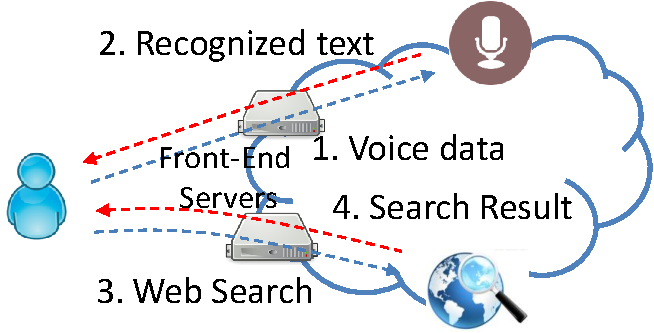
\includegraphics[width=0.8\linewidth]{voice_search_process}
	\caption{Voice search engine infrastructure.}
	\label{fig:voice_search}
\end{figure}

\subsection{Measurements and Metrics}

We divide the analysis framework into two parts according to which phase the flow belongs to. The reasons are as follows. First, the two parts are located in different flows of two independent phases. Second, the performance in the two phases is affected by different factors. Servers act as receivers in voice uploading phase, and senders in web search phase. Essentially, as a sender-driven transmission protocol, TCP's transmission performance is basically affected by the efficiency that sender could handle congestion events, as well as the capability that receiver could receive data.Last but not least, different factors could be collected in the two phases. In voice recognition, at most three RTT's could be measured, in establishing, terminating connections, as well as transmitting the ``recognized text'' packet. Besides, we could not distinguish whether a packet is retransmitted or reordered by network. However, in web search phase, plenty of RTT's could be measured. Furthermore, we could identify each packet loss, retransmission, or reordering event in web search phase.

We mainly investigate the impact of network quality on the user-perceived performance in voice search. Thus, the time unrelated to network factors is not considered, such as time consumed by voice recognition.

\begin{figure}[th]
\centering
\begin{subfigure}[b]{0.8\linewidth}
	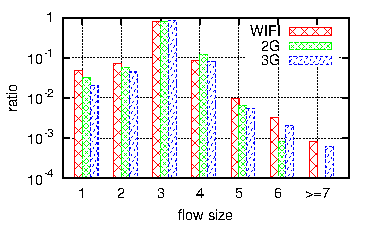
\includegraphics[width=\textwidth]{voice_flow_size}
\caption{Voice recognition}
\label{fig:voice_flow_size}
\end{subfigure} \\
%\vspace{0.1in}
\begin{subfigure}[b]{0.8\linewidth}
	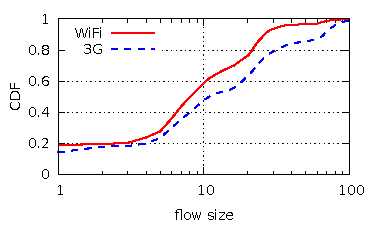
\includegraphics[width=\textwidth]{web_flow_size}
\caption{Web Search}
\label{fig:web_flow_size}
\end{subfigure}
\caption{The distribution of flow sizes (in packet) in the two phases.}
\label{fig:flow_size}
\end{figure}

Figure~\ref{fig:flow_size} plots the distribution of flow sizes in the two phases. It is worth noting that the packet carrying text in voice recognition and the HTTP GET packet in web search are not calculated in the flow size. Figure~\ref{fig:voice_flow_size} shows the ratio of flow with various sizes, in which the $y$-axis is drawn in log scale. From the figure, nearly all flows contain no more than 6 data packets. The initial congestion window in current Android TCP/IP stack is set to 10 segments\cite{dukkipati2010argument}, which means the voice data could be transmitted in the first congestion window. Figure~\ref{fig:web_flow_size} shows the Cumulative Distribution Function (CDF) of flow sizes in web search. From the figure, all flows are with less than 100 data packets, in which a large fraction of flows (64\%) are with size in range between 5 and 30 packets. There are also flows with no search result, resulting in one data packet in the flow, which occupy 15\% of flows.

\begin{figure}[th]
\centering
\begin{subfigure}[b]{0.8\linewidth}
	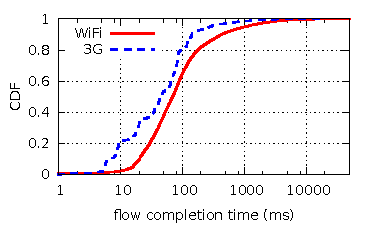
\includegraphics[width=\textwidth]{voice_finish_time}
\caption{Voice recognition}
\label{fig:voice_finish_time}
\end{subfigure} \\
%\vspace{0.1in}
\begin{subfigure}[b]{0.8\linewidth}
	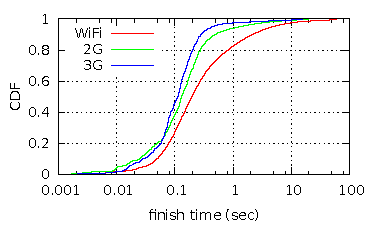
\includegraphics[width=\textwidth]{web_finish_time}
\caption{Web search}
\label{fig:web_finish_time}
\end{subfigure}
\caption{CDFs of time consumed in the two phases.}
\label{fig:finish_time}
\end{figure}

Figure~\ref{fig:finish_time} shows the CDF of the time consumed in the two phases. From Figure~\ref{fig:voice_finish_time}, we could see that more than 60\% of voice recognition flows experience latency of less than 100~ms. However, a non-negligible fraction of flows (3\% in CT and CU, and 11\% in CM) experience more than 1 second to upload the voice data. As in most of flows, mobile client could transmit all the voice data in the initial congestion window, the relatively large time values show that the voice recognition performance degrades due to network factors, like large RTT, packet loss, and TCP stack inefficiency. To depict the user-perceived performance in voice recognition and web search, we define performance metric $finish\_time$, measured in seconds. This metric represents the duration from client initiates to establish the connection till the time that the last byte is acknowledged. Note that mobile client is the sender in voice recognition and is the receiver in web search. As we could not determine the exact time when the SYN packet is transmitted in voice recognition, we use the time when the SYN packet is received to approximate the beginning of the duration.

Figure~\ref{fig:web_finish_time} shows the CDF of $finish\_time$ of web search flows. In the figure, 38\% of flows experience $finish\_time$ less than 0.1 second. However, 7\% of flows experience $finish\_time$ more than 1 second. Furthermore, about 3\% of flows are with $finish\_time$ more than 10 seconds, which is a great performance degradation. As shown in Figure~\ref{fig:web_flow_size}, the flow size in web search ranges from 1 to 100 packets. This means that the data could be transmitted in 1 RTT at least, and more than 4 RTT at most. Considering the various flow sizes, the metric $finish\_time$ could not portray the efficiency that the data is delivered. To eliminate the affect of flow size, we introduce one more performance metric $trans\_speed$, defined as the average time to transmit a data packet. The metric $trans\_speed$ could be represented as $\frac{finish\_time}{\#(pkts)}$.

To evaluate the impact of network quality on user experience in voice search, we mainly consider the following network factors in the analysis:

\begin{itemize}
\setlength{\itemsep}{-8pt}
\setlength{\topsep}{-8pt}
	\item {Access Type: } Mobile client could issue the voice search service via 2G/3G/4G or WiFi network. Different access types exhibit different network characteristics. For example, compared with WiFi network, the latency in cellular network is larger, while packet loss or reordering event is rarer. \\
	\item {Round Trip Time (RTT): } If two senders have the same congestion window size, the one with smaller RTT will receive acknowledgments in shorter time, thus could transmit more data per unit time, resulting smaller $finish\_time$. \\
	\item {Packet Loss / Packet Reordering: } Both packet loss and packet reordering could affect the transmission efficiency. Packet loss leads to reduction of sender's congestion window. Though packet reordering does not reduce congestion window, it will prevent congestion window from growing and may trigger spurious retransmission. \\
	\item {Timeout Retransmission (RTO): } Timeout retransmission could be triggered due to insufficient number of duplicate acknowledgments under packet loss~\cite{rfc6675}. The RTO timer could be set to more than 200~ms in current Linux/Android implementation, and will be doubled if the retransmitted packet is dropped, which is exceptionally high in short flows~\cite{flach2013reducing}.\\
\end{itemize}

To summarize, we mainly investigate the impact of network factors, including \emph{access type}, \emph{RTT}, \emph{network event}, \emph{timeout retransmission}, on user-perceived performance in voice search process, including $finish\_time$, $trans\_speed$.

\subsection{Analysis Methodology}

To unveil the impact of network factors on user-perceived performance in voice search service, we introduce a collection of analysis methodologies to determine which factors matter the most, and how much a factor affects the performance quantitatively.

\subsubsection{Correlation Coefficient}

Correlation coefficient is the natural approach to depict the interaction between two variables. Here we use Pearson Correlation Coefficient (PCC) to quantify the magnitude of relationship between network factors and performance metrics in voice search service. PCC is a measure of linear correlation between two numeric variable $x$ and $y$. PCC determines the correlation coefficient via formula $\text{corr}(x,y) = \frac{\text{cov}(x,y)}{\text{dev}(x) \text{dev}(y)}$, where $\text{cov}(.,.)$ is the covariance function, and $\text{dev}(.)$ is the standard deviation. The correlation coefficient ranges from -1 to 1, where -1 represents total negative correlation, 0 is no correlation, and -1 is total positive correlation.

We group the data into bins with appropriate interval values, like 40~ms in RTT, and compute the mean performance value. The bin index and the average value in each bin are the input of PCC to investigate their relation. We use the binned data instead of the original data due to the following reasons. Instead of studying performance in specific flows, we, in this paper, attempt to understand how network factors impact the performance metrics. Thus we bin the data to eliminate the noise in data. Besides, the binned value is more direct viewing and easier to compute.

\subsubsection{Quasi-Experimental Design (QED)}

To casually depict the impact of network factors on user-perceived performance, we adopt controlled experiment methodology ``Quasi-Experimental Design'' (QED) \cite{krishnan2013video}. The basic idea of QED is to investigate the significance of a factor $x$ by varying this factor while controlling other factors as invariable.

The process of QED could be exemplified as follows. To understand the impact of packet loss event on finish time, we first bin the flows into different groups, $\{ F_0, F_1, F_2, \cdots, F_n \}$, by measuring how many packets are lost in the flow, where the index represents the number of lost packets. To investigate the impact of various number of lost packets, we take $F_0$ (\ie with no lost packet) as the baseline. For any flow $u$ in $F_0$, we randomly choose a flow $v$ which has similar properties with flow $u$: access type, RTT and flow size. If there is such a flow $v$, we record $o_{u,v} = (finish\_time_{u} - finish\_time_{v})$. Thus at most $|F_0|$ $(u,v)$ pairs could be found in $F_0$ and $F_i$. Compared with $F_0$, when the number of lost packets is $i$, the introduced performance degradation is $D_{i} = \sum o_{u,v} / m$.